\documentclass[11pt]{article}

\usepackage[margin=1in]{geometry}
\usepackage{graphicx}
\usepackage{booktabs}
\usepackage{float}
\usepackage{amsmath}
\usepackage{amssymb}
\usepackage{xcolor}
\usepackage{hyperref}
\usepackage{listings}

\title{\textbf{Assignment Report}}
\author{%
    Your Name\\
    Email: Your Official Email
}
\date{\today}

\lstset{
    basicstyle=\ttfamily\small,
    breaklines=true,
    frame=single,
    columns=fullflexible
}


\begin{document}

\maketitle

\tableofcontents
\newpage

\section{Part 1}

\subsection{Design}

Describe the design of your solution for Part 1.

Explain the overall workflow of your implementation and how the different
components interact. The description should contain enough detail that
another knowledgeable programmer could reproduce your implementation.

\subsection{Results}

Present the timing results for Part 1.

The primary result should be a line graph showing speedup relative to the
reference implementation.

\begin{figure}[H]
    \centering
    % Replace with your actual figure.
    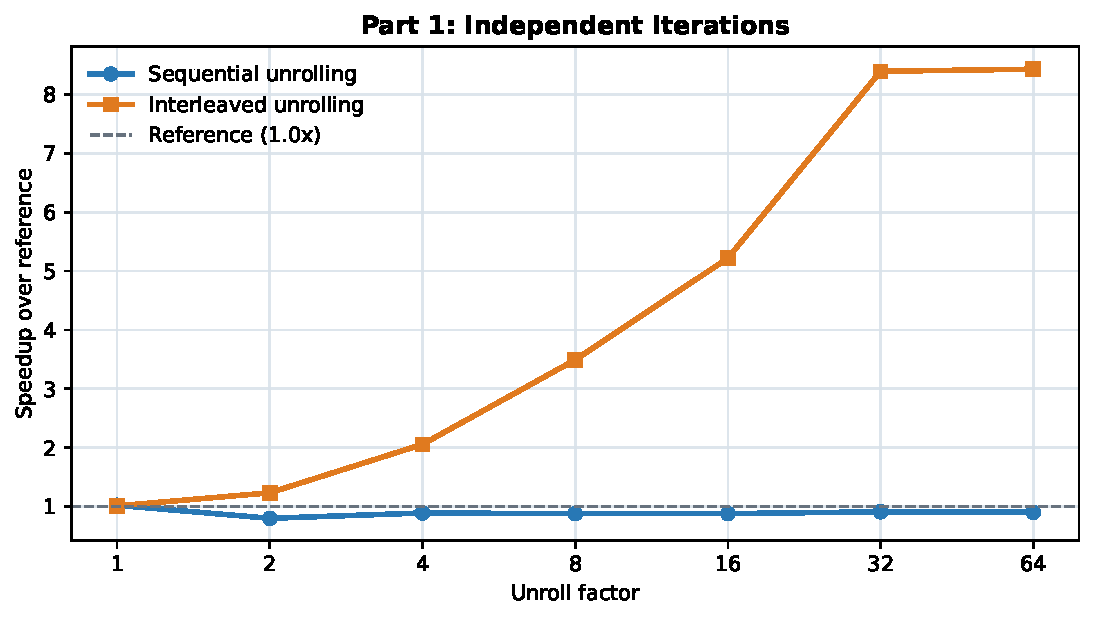
\includegraphics[width=0.8\textwidth]{part1_results.pdf}
    \caption{Part 1 speedup relative to the reference implementation.}
    \label{fig:part1-results}
\end{figure}

The x-axis should show the parameter being varied, and the y-axis should
show speedup relative to the reference implementation.

You should also include a table containing the raw timing measurements.
Here is a sample table.

\begin{table}[H]
    \centering
    \caption{Part 1 timing results.}
    \label{tab:part1-results}
    \begin{tabular}{cccc}
        \toprule
        Parameter & Reference &  Sequential & Interleaved\\
        \midrule
        \bottomrule
    \end{tabular}
\end{table}

\subsection{Analysis}

Analyze the results from Part 1.

Explain:

\begin{itemize}
    \item What trends you observe in the results.
    \item Why the performance changes as the parameter is varied.
    \item Why the optimized implementation differs from the reference implementation.
    \item Any performance limitations or unexpected results.
    \item Whether the results agree with your expectations.
\end{itemize}


\section{Part 2}

\subsection{Design}



\subsection{Results}


\subsection{Analysis}


\section{Part 3}

\subsection{Design}



\subsection{Results}

\subsection{Analysis}

\end{document}